\documentclass[border=2pt]{standalone}
\usepackage{tikz}
\usepackage{pgfplots}
\usetikzlibrary{arrows.meta,positioning}
\pgfplotsset{compat=1.18}
\definecolor{mprimary}{HTML}{2C3E6B}
\definecolor{maccent}{HTML}{C8A951}
\definecolor{mgood}{HTML}{5B8C6B}
\definecolor{mgray}{HTML}{9E9E9E}
\definecolor{mlight}{HTML}{EEF0F5}
\definecolor{mlightsage}{HTML}{E5EDE8}
\begin{document}
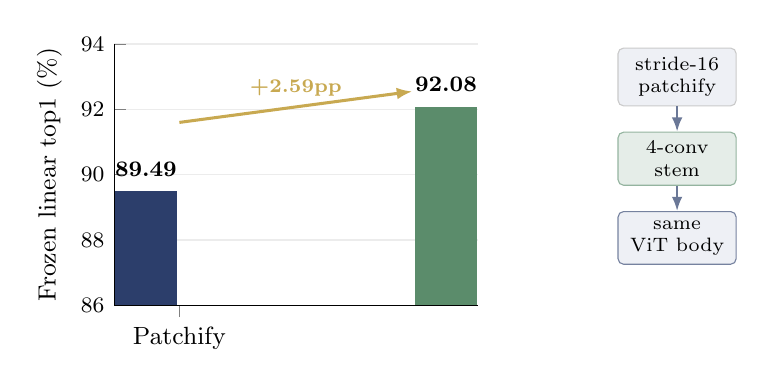
\begin{tikzpicture}
\begin{axis}[
    width=6.2cm, height=4.9cm,
    ybar, bar width=0.78cm,
    ylabel={Frozen linear top1 (\%)},
    ymin=86, ymax=94,
    ymajorgrids=true,
    grid style={mgray!20},
    axis x line*=bottom,
    axis y line*=left,
    symbolic x coords={Patchify,{Conv-stem}},
    xtick=data,
    xticklabel style={font=\small, align=center},
    tick label style={font=\footnotesize},
    label style={font=\small},
    nodes near coords,
    point meta=explicit symbolic,
    nodes near coords style={font=\footnotesize\bfseries, yshift=2pt},
    enlarge x limits=0.28]
  \addplot[draw=none, fill=mprimary] coordinates {(Patchify,89.49) [89.49]};
  \addplot[draw=none, fill=mgood] coordinates {({Conv-stem},92.08) [92.08]};
  \draw[maccent, line width=1.1pt, -{Latex[length=2mm]}] (axis cs:Patchify,91.6) -- node[above, font=\scriptsize\bfseries] {+2.59pp} (axis cs:{Conv-stem},92.55);
\end{axis}
\node[draw=mgray!55, fill=mlight, rounded corners=2pt, minimum width=1.5cm, minimum height=0.52cm, font=\scriptsize, align=center] (p) at (7.15,2.9) {stride-16\\patchify};
\node[draw=mgood!65, fill=mlightsage, rounded corners=2pt, minimum width=1.5cm, minimum height=0.52cm, font=\scriptsize, align=center, below=0.32cm of p] (c) {4-conv\\stem};
\node[draw=mprimary!65, fill=mlight, rounded corners=2pt, minimum width=1.5cm, minimum height=0.52cm, font=\scriptsize, align=center, below=0.32cm of c] (v) {same\\ViT body};
\draw[-{Latex[length=1.8mm]}, thick, mprimary!70] (p) -- (c);
\draw[-{Latex[length=1.8mm]}, thick, mprimary!70] (c) -- (v);
\end{tikzpicture}
\end{document}
